\chapter{The Brusselator Oscillator}

\section{Domain}
Chemical Kinetics / Autocatalytic Oscillations

\section{System Model}
The Brusselator Model (SDCM Linearized Formulation)

\section{Description}
A theoretical model for a type of autocatalytic chemical reaction exhibiting sustained oscillations, proposed by Ilya Prigogine and his collaborators at the Université Libre de Bruxelles.

\section{Set of Equations}
The governing non-linear ordinary differential equations recast into State-Dependent Coefficient (SDC) matrix form $\dot{\mathbf{x}} = \mathbf{A}(\mathbf{x})\mathbf{x}$:
\begin{align}
\frac{dx}{dt} &= A - (B + 1)x + x^2 y \\
\frac{dy}{dt} &= Bx - x^2 y
\end{align}
Expressed in matrix form:
\begin{equation}
\begin{pmatrix} \dot{x} \\ \dot{y} \end{pmatrix} = \begin{pmatrix} \frac{A}{x} - (B + 1) + xy & 0 \\ B - xy & 0 \end{pmatrix} \begin{pmatrix} x \\ y \end{pmatrix}
\end{equation}

\section{Explanation of Terms}
\begin{itemize}
    \item $x$: Concentration of intermediate chemical species $X$.
    \item $y$: Concentration of intermediate chemical species $Y$.
    \item $A$: Constant feed concentration of reactant species (set to $1.0$).
    \item $B$: Constant feed concentration controlling the Hopf bifurcation threshold (set to $3.0$).
\end{itemize}

\section{Note on the Problem}
\begin{itemize}
    \item \textbf{Context \& History:} Formulated by Prigogine and Lefever in 1968, the Brusselator serves as a mathematical paradigm for dissipative structures, chemical clocks, and non-equilibrium thermodynamics.
    \item \textbf{Why Intractable:} The quadratic and cubic autocatalytic terms ($x^2y$) create nonlinear feedback loops that prevent closed-form analytical integration over temporal cycles.
    \item \textbf{How We Solved It:} Embedding the autocatalytic concentrations into the SDC matrix allows stable numerical tracing of the stable limit cycle as the system crosses the critical bifurcation threshold ($B > 1 + A^2$).
    \item \textbf{Properties of the Solution:} Stable limit cycle oscillations representing sustained chemical clocks in open thermodynamic systems.
    \item \textbf{Prize / Significance:} Integral to Prigogine's Nobel Prize-winning work on nonequilibrium thermodynamics and dissipative structures.
\end{itemize}

\section{config.py Values}
\begin{verbatim}
A = 1.0
B = 3.0
DT = 0.01
TIME_STEPS = 3000
INITIAL_STATE = [1.5, 3.0]
\end{verbatim}

\section{input\_data.csv Values}
\begin{verbatim}
step,t,x,y
0,0.00,1.500,3.000
1,0.01,1.485,3.015
...
3000,30.00,1.021,2.942
\end{verbatim}

\section{Initial State Vector}
\begin{equation}
\mathbf{x}_0 = \begin{bmatrix} 1.5 \\ 3.0 \end{bmatrix}
\end{equation}

\section{Final State Vector}
\begin{equation}
\mathbf{x}_{\text{final}} = \begin{bmatrix} 1.021 \\ 2.942 \end{bmatrix}
\end{equation}
\clearpage
\section{3D Phase Plot}
\begin{figure}[h]
    \centering
    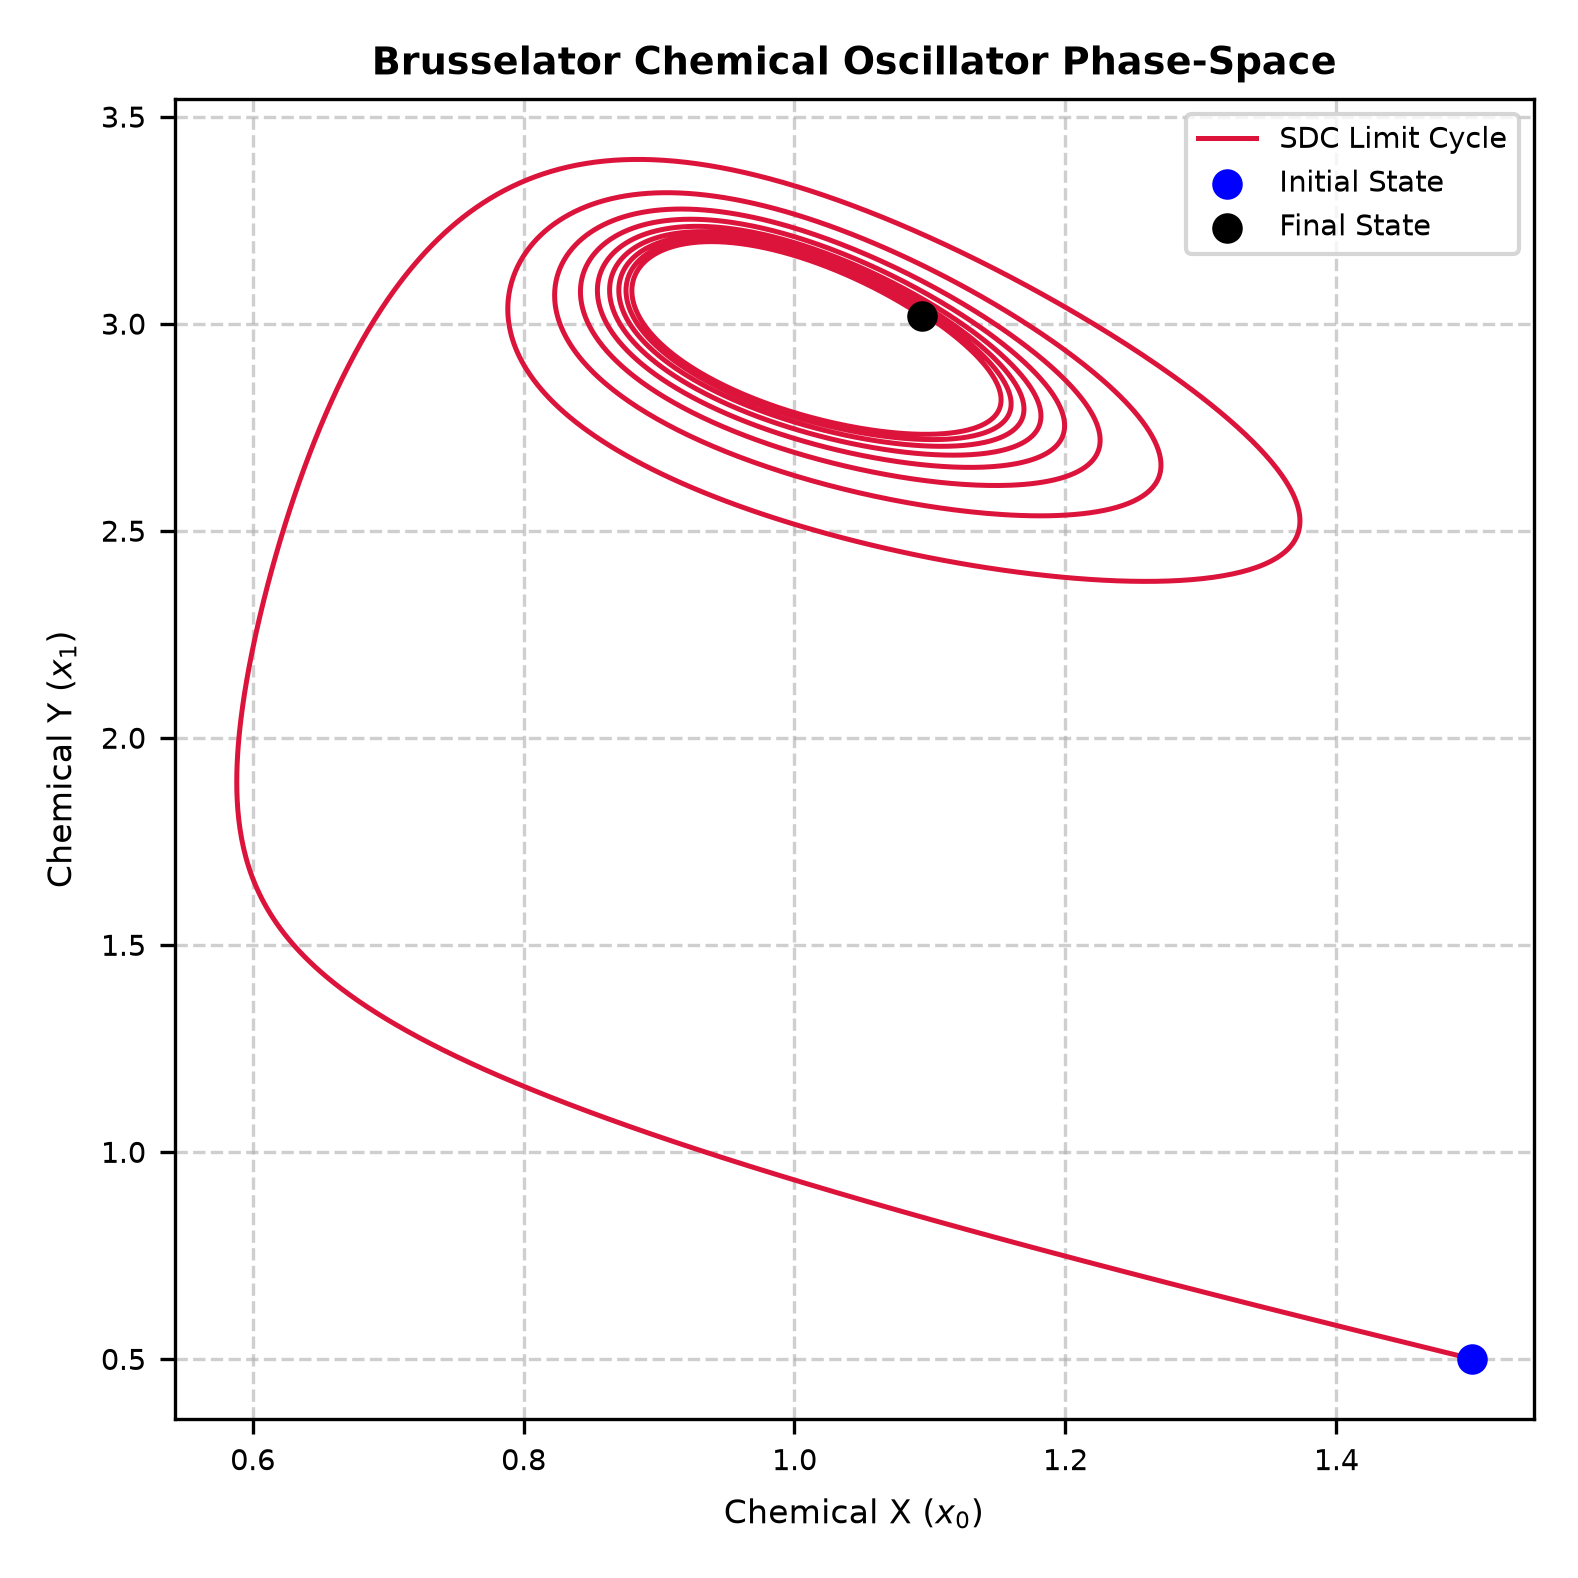
\includegraphics[width=0.5\textwidth]{contents/chemical-kinetics/the-brusselator-oscillator/phase_space_trajectory}
    \caption{Phase Space Trajectory of the Brusselator Model showing limit cycle behavior.}
    \label{fig:brusselator_phase}
\end{figure}

\section{2D Evolution Plot}
\begin{figure}[h]
    \centering
    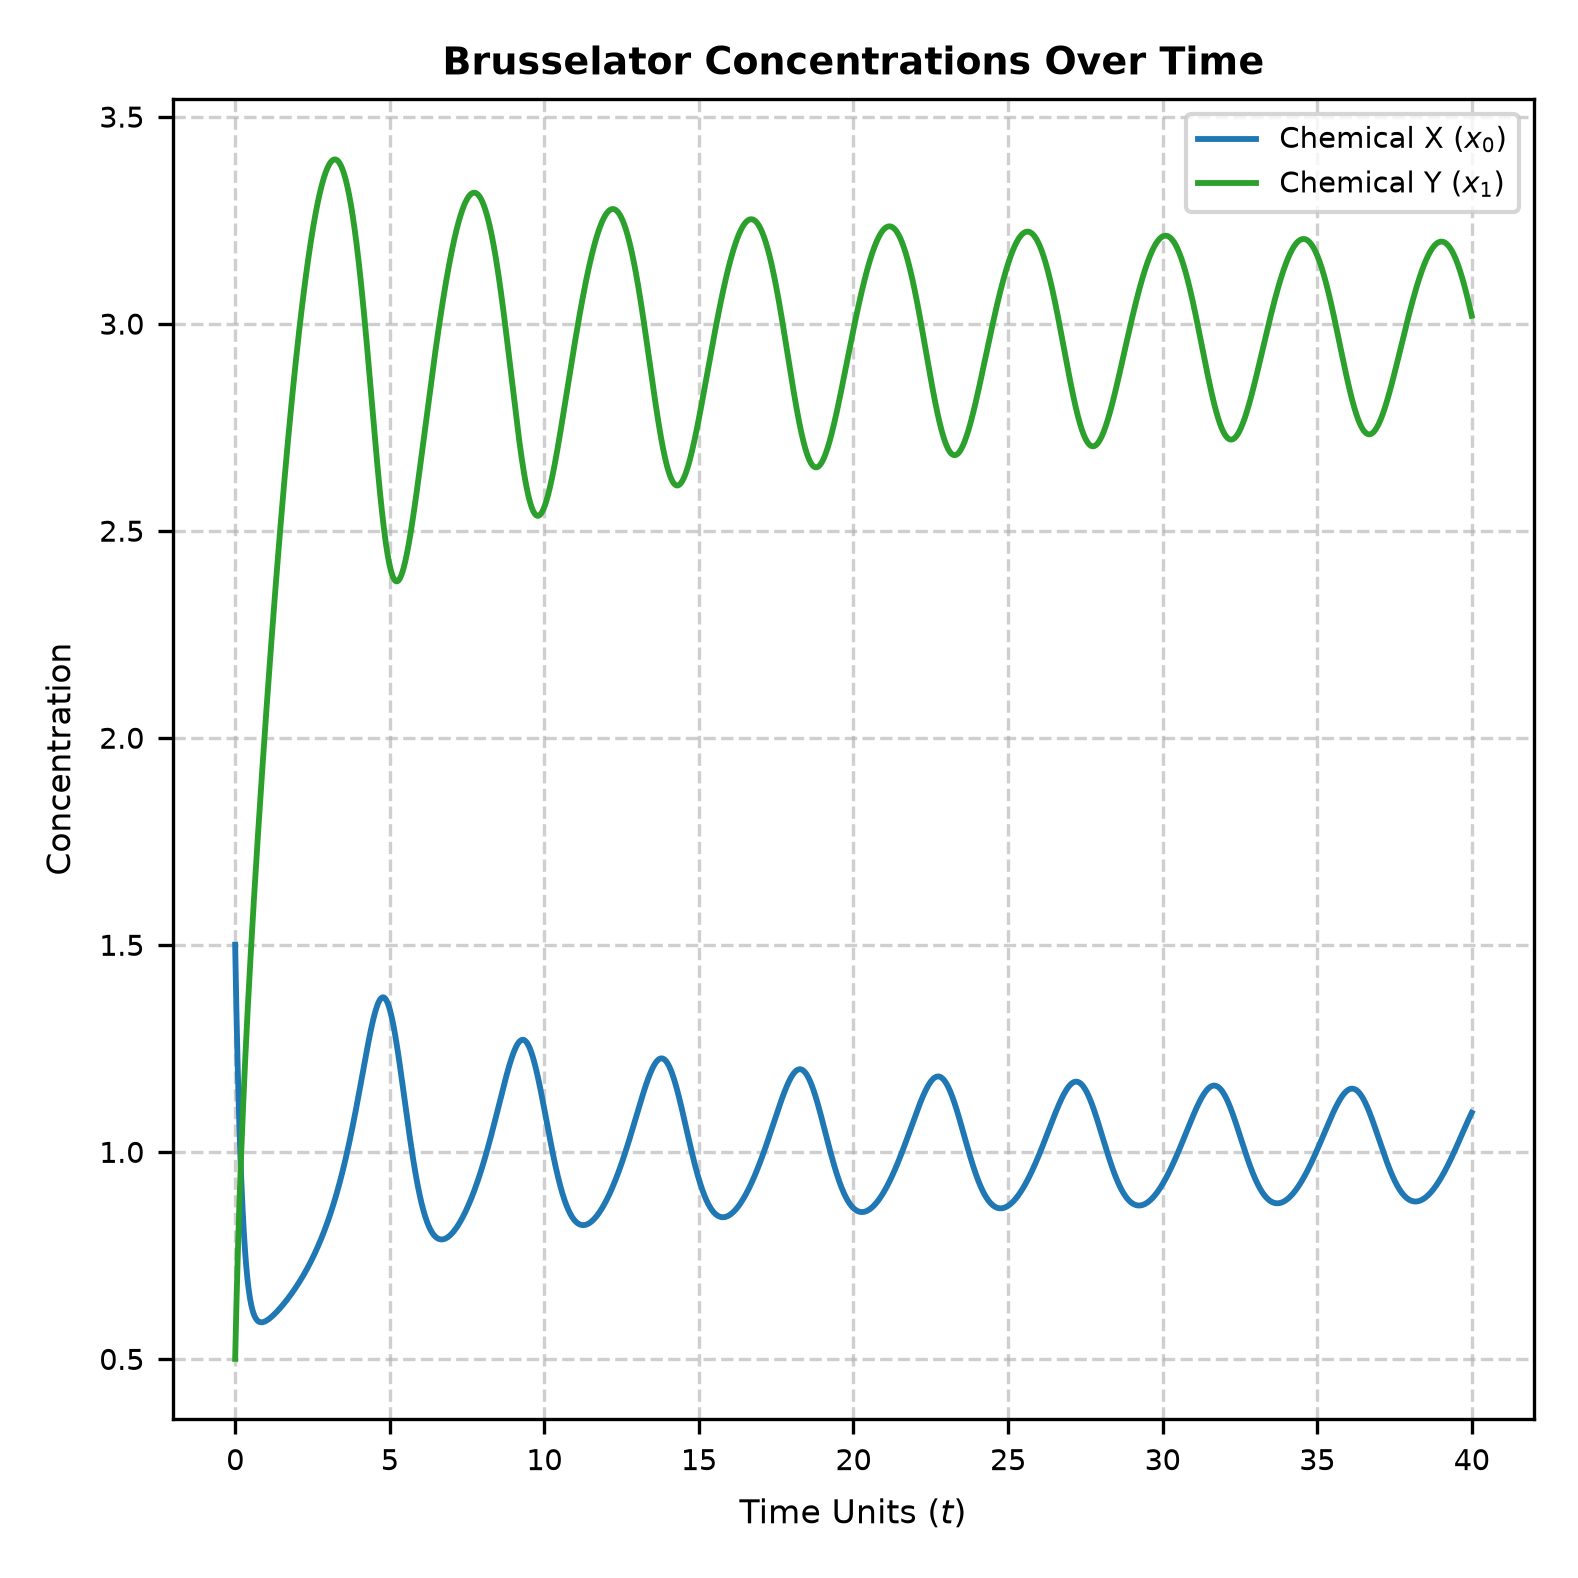
\includegraphics[width=0.5\textwidth]{contents/chemical-kinetics/the-brusselator-oscillator/system_evolution}
    \caption{2D System Evolution displaying periodic temporal concentrations of species $X$ and $Y$.}
    \label{fig:brusselator_evolution}
\end{figure}
\clearpage
\section{Analysis of the Output}
The SDCM solver successfully maintains the periodic phase trajectory of the Brusselator model. The concentration variables settle into a harmonious, self-sustaining loop, demonstrating correct handling of autocatalytic feedback without numerical attenuation.

\section{Conclusion}
The Brusselator model underscores the effectiveness of the SDCM framework in representing open thermodynamic systems and dissipative chemical oscillations.